\documentclass[a4paper,12pt]{article}
\usepackage{xcolor}
\usepackage{tikz}
\usepackage{geometry}
\usepackage{courier}   % Fonte monoespaçada
\usepackage{microtype} % Permite ajustar espaçamento entre letras
\microtypesetup{expansion=false}


% Definir margens
\geometry{top=2cm, bottom=2cm, left=2cm, right=2cm}

\begin{document}

% Criar fundo preto com grade
\begin{tikzpicture}[remember picture, overlay]
    \draw[step=0.3cm, gray!15] (current page.south west) grid (current page.north east);
\end{tikzpicture}

\ttfamily       % Fonte monoespaçada
\fontsize{14}{0}\selectfont  % Tamanho da fonte
\baselineskip=0.3cm         % Altura da linha igual ao passo da grade


% Ajustar espaçamento entre letras para que cada caractere ocupe 0.5cm
\textls[27]{TEXTO} % Valor ajustado experimentalmente

\end{document}